Für den Fall, dass beim Authentisierungsvorgang keine Bluetooth-Verbindung 
zwischen App und Browser hergestellt werden kann, gibt es eine alternative 
Lösung. In Abb. \ref{fig: konzept fallback} ist der Ablauf des alternativen 
Authentisierungsvorgangs dargestellt.
\\\\
\begin{figure}
    \centering
    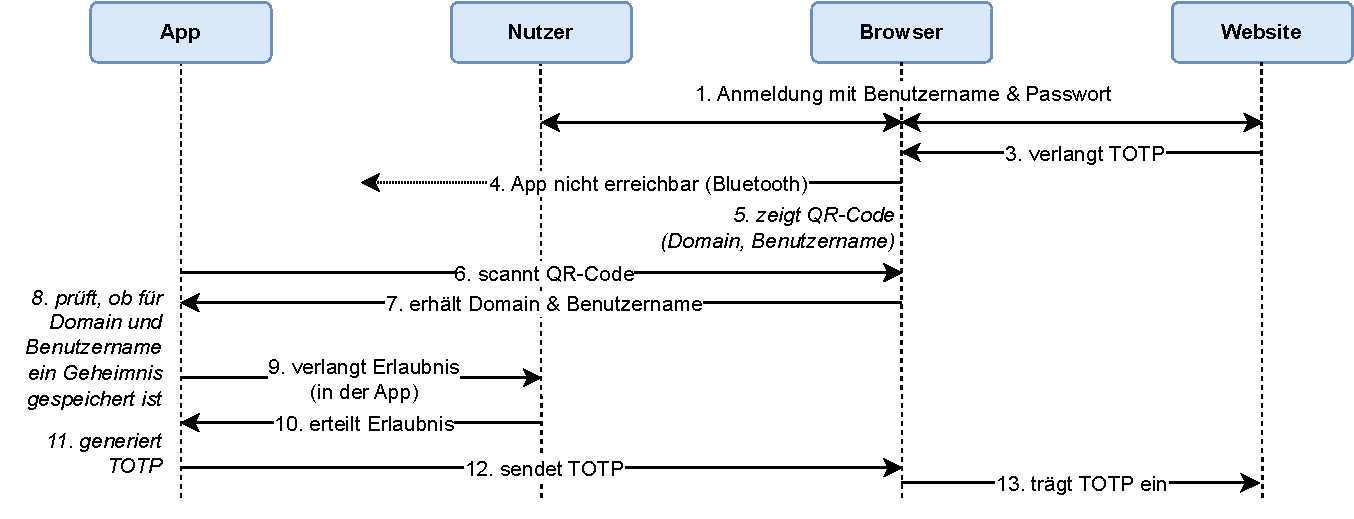
\includegraphics[width=1\linewidth]{figures/konzept_login_fallback.pdf}
    \caption[Fallback des Konzepts zu einem neuen TOTP-Verfahren]{Alternativer Authentisierungsvorgang (Fallback) des Konzepts zu einem neuen TOTP-Verfahren}
    \label{fig: konzept fallback}
\end{figure}
Bis auf die Schritte 4, 5, 6 und 9 sind alle Schritte identisch mit den 
entsprechenden Schritten des normalen Authentisierungsvorgangs. In Schritt 3 
erkennt der Browser, dass das TOTP verlangt wird und versucht eine 
Bluetooth-Verbindung zur App herzustellen. In diesem Fall scheitert der 
Verbindungsaufbau und der Browser bietet dem Nutzer den alternativen 
Authentisierungsvorgang an. Dazu zeigt der Browser einen QR-Code an, der 
letztlich nur den Benutzernamen und die Domain enthält (Schritt 5). Wichtig ist 
hier zu erwähnen, dass der Browser den QR-Code anzeigt und nicht die Website. 
Sollte es eine Phishing-Website sein, könnte sie im QR-Code die Domain der echten 
Website angeben, die sie imitiert. Daher vertraut man der Website nicht. Der Nutzer 
scannt den QR-Code (Schritt 6) und es öffnet sich die App. Nun hat die App die 
Domain und den Benutzernamen erhalten und es wird wie beim normalen 
Authentisierungsvorgang fortgefahren. Ausnahme sei Schritt 9. Da die App momentan 
schon geöffnet ist, kann sie direkt den Nutzer um Erlaubnis fragen, um das TOTP 
an den Browser zu senden. Es muss nicht extra eine Notification erstellt werden. 
\\\\
Es existiert noch eine Schwachstelle bei Schritt 3, indem man sich der potentiellen 
Unwissenheit des Nutzers bedient. Eine Phishing-Website könnte anstatt eines 
TOTP-Eingabeelements einen QR-Code anzeigen und den Nutzer auffordern, diesen zu 
scannen. Der QR-Code enthält die Domain der echten Website und den eben eingegebenen 
Benutzernamen. Der Nutzer weiß aber in diesem Szenario nicht, dass er keine QR-Codes 
von der Website scannen darf bei der Authentisierung, also scannt er den QR-Code. Die 
App würde ihm nun das TOTP anzeigen und er würde es unwissentlich in die 
Phishing-Website eingeben. Es ist denkbar, bei einer früheren Verbindung zwischen 
Browser und App asymmetrische Schlüssel auszutauschen und Informationen im QR-Code zu 
signieren, die dann von der App beim Scan entschlüsselt und verifiziert werden. So 
weiß die App, dass der QR-Code vom Browser stammt. Denn die Phishing-Website kennt 
nicht den Schlüssel des Browsers und kann demnach keinen gültigen QR-Code erstellen. 
Allerdings bleibt die Frage offen, wie man gegen dieses Szenario vorgeht, wenn der 
Nutzer den vorliegenden Browser in Kombination mit seiner App das erste Mal nutzt. 